\documentclass[a4paper,titlepage]{article}
\usepackage[utf8]{inputenc}
\usepackage[T1]{fontenc}
\usepackage[magyar]{babel}
\usepackage{amsmath}
\usepackage{float}
\usepackage{graphicx}

\newcommand{\Ai}[1]{\mathrm{Ai\left(#1\right)}}
\newcommand{\Bi}[1]{\mathrm{Bi\left(#1\right)}}
\newcommand{\Ti}[1]{\mathrm{Ti\left(#1\right)}}


\begin{document}
\section{Leírás}
	Kvantummechanikai iskolapélda a homogén térbe helyezett egydimenziós
	részecske. Ezt három dimenzióra kiterjesztve és két fal közé zárva
	keressük az energia sajátállapotokat. Annyi előrelátható, hogy a nyílt
	vagy félig nyílt esetekben használható, reguláris Airy függvény itt nem
	elegendő a megoldáshoz, ennyiben túlmegyünk a tankönyvi feladaton. Az
	aszimptotikus függvényalakok segítségével előállítjuk a magasan
	gerjesztett állapotok energiáit és hullámfüggvényeit, s ezeket
	összehasonlítjuk a közvetlenül a Bohr--Sommerfeld-módszerrel kapott
	eredménnyel. Numerikusan szemléltetjük fizikailag érdekes kezdőállapotok
	időfejlődését. Vizsgáljuk a rezolvenst és az állapotsűrűséget, továbbá a
	sokrészecske rendszerekre való általánosítás lehetőségét.
	
	Egydimenziós, $m$ tömegű, lineáris $F x$  potenciálban mozgó kvantumos részecskét zárjunk $L$ hosszú, merev falú dobozba (ekvivalens a padló és mennyezet között függőlegesen pattogó kvantum labdával).
	A stacionárius Schrödinger-egyenletből kiindulva, a határfeltételek figyelembe vételével, írjuk fel az energia sajátértékeket meghatározó szekuláris egyenletet, melyet oldjunk meg numerikusan. Ábrázoljuk az alacsonyabb nívókat a doboz méretének változtatása mellett, és szemléltessük grafikusan a stacionárius hullámfüggvényeket.  A szekuláris egyenletben fellépő függvények aszimptotikáinak ismeretében a magasabb nívókra próbáljunk egyszerűbb implicit formulát adni. Végezzük el a szemiklasszikus kvantálást is, hasonlítsuk össze az előző közelítő eredménnyel, és numerikusan néhány, az egzakt egyenletből kapott nívóval.

	További kérdések:  (a) Számítsuk ki a nívókat expliciten, kicsiny $L$-ek mellett. (b) Mely paraméterek mellett esik egybe $F L$ éppen az alapállapoti energiával?  (Ilyenkor a klasszikus labda éppen eléri a mennyezetet.)
	(c) Mutassuk meg, hogy e határesetnél kisebb $L$ belméret mellett minden nívó
	$F L$ fölé esik.
	(d) Írjuk fel a szemiklasszikus stacionárius hullámfüggvényeket, s grafikusan hasonlítsuk össze őket az egzaktakkal -- mikor jó a közelítés?
	(e) Írjuk fel a kicsiny L melletti hullámfüggvényeket expliciten, ezeket szintén hasonlítsuk össze a valódiakkal.
	
	-Miért nem Rodnik osztályba tartozik
	
	-20-as képlet lépcsőfüggvény
	
	-klasszikus út
	
	-fx, fy = 0 külön tárgyalás
	
	-program leírása
\section{Schrödinger}
	A probléma egy 1D doboba zárt résecske homogén erőtérben. $F(x)=-F$, azaz $V(x) = Fx$.
	Az egyenlethez tartozó határfeltételek, ha a doboz hossza $L$:
	\begin{equation}
		\psi \big\rvert_0 = \psi \big \rvert_L = 0
	\end{equation}
	A megoldandó időfüggetlen Schrödinger-egyenlet:
	\begin{equation}
		-\frac{\hbar^2}{2m}\frac{d^2\psi}{dx^2} + Fx\psi = E\psi
	\end{equation}
	\begin{equation}
		\frac{d^2\psi}{dx^2} - \frac{2mFx}{\hbar^2}\psi = -\frac{2mE}{\hbar^2}\psi
	\end{equation}
	\begin{equation}
		\frac{d^2\psi}{dx^2} - \left(\frac{2mF}{\hbar^2}x - \frac{2mE}{\hbar^2}\right)\psi = 0
	\end{equation}
	Az Airy egyenlet ilyen alakra hozható a változó affin lineáris transzformációjával:
	\begin{equation}
		\frac{d^2y}{dx^{\prime 2}} - x^\prime y = 0
	\end{equation}
	$x^\prime = ax - b$, azaz $\frac{d}{dx} = a\frac{d}{dx^\prime}$:
	\begin{equation}
		\frac{d^2y}{dx^2} - \left(a^3x - a^2b\right)y = 0
	\end{equation}
	Az együtthatók összevetése alapján $a = \sqrt[3]{\frac{2mF}{\hbar^2}}$ és $b = \sqrt[3]{\frac{2m}{\hbar^2F^2}}E$. Így a Schrödinger-gyenlet megoldása:
	\begin{equation}
		\psi(x) = y(x^\prime) = y\left(\sqrt[3]{\frac{2mF}{\hbar^2}}x - \sqrt[3]{\frac{2m}{\hbar^2F^2}}E\right)
	\end{equation}
	, ahol $y(x) = \alpha \Ai{x} + \beta \Bi{x}$.
	A $\psi \big\rvert_0 = 0$ feltételből következik, hogy $\psi \propto \Bi{-b}\Ai{ax-b} - \Ai{-b}\Bi{ax-b}$. A második határfeltétel pedig meghatározza a lehetséges energiákat. A feltétel:
	\begin{equation}
		\Bi{-b}\Ai{aL-b} - \Ai{-b}\Bi{aL-b} = 0
	\end{equation}
	\begin{equation}
		\label{box_energiaszintek_egyenlet}
		\Ti{aL-b} - \Ti{-b} = 0
	\end{equation}
	\begin{equation}
		\Ti{\sqrt[3]{\frac{2mF}{\hbar^2}}L - \sqrt[3]{\frac{2m}{\hbar^2F^2}}E} - \Ti{-\sqrt[3]{\frac{2m}{\hbar^2F^2}}E} = 0
	\end{equation}
	\begin{figure}[H]
		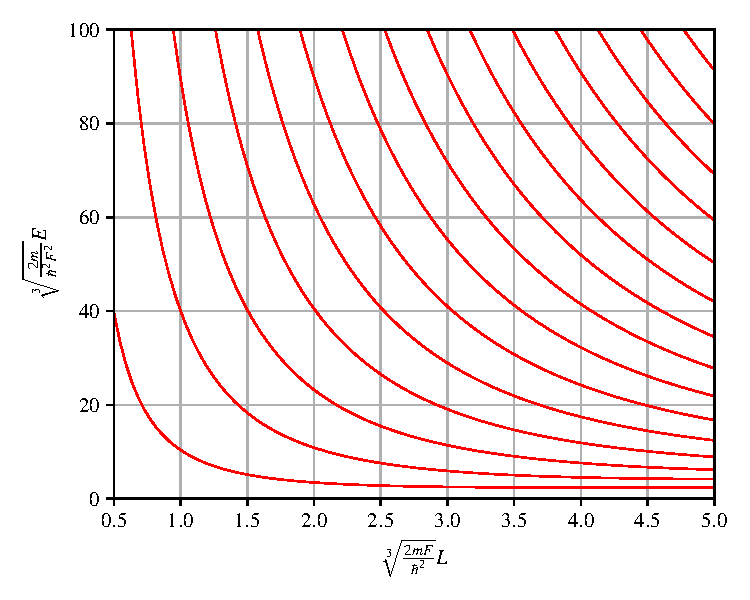
\includegraphics[scale=1]{./figs/energiaszintek.pdf}
		\caption{Energiaszintek $L$ függvényében}
		\label{box_energiaszintek_abra}
	\end{figure}
	Amikor $FL \ll \frac{\pi^2\hbar^2}{2mL^2}$, a potenciál jól közelíthető konstans potenciállal, mivel az alapállapot energiájához képest is elhanyagolható a lineáris potenciál eltérése a konstans potenciáltól. Eben a esetben $E \propto n^2$. $E \ll FL$ esetben az energiaszintek jó közelítéssel konstanssá válnak. Ennek az oka, hogy $\lim_{L \to \infty}\psi(x) = \alpha \Ai{ax-b}$, mert a $Bi(x)$ exponenciálisan növekszik nagy $x$-ek esetén. Ebben az eseten az energiaszinteket a $\Ai{- \sqrt[3]{\frac{2m}{\hbar^2F^2}}E} = 0$ egyenlet határozza meg. Ezeket az aszimptotikus viselkedéseket \aref{box_energiaszintek_abra}. ábra jól mutatja.
    
    TODO: link 1D videóról

\section{Kvantumos közelítése}
	$x \rightarrow \infty$ aszimptotikus alak:
	\begin{equation}
		\Ai{-x} = \frac{1}{\sqrt{\pi}x^{1/4}}\cos\left(\frac{2}{3}x^{3/2} - \frac{\pi}{4}\right) + \mathcal{O}\left(x^{-5/4}\right)
	\end{equation}
	\begin{equation}
		\Bi{-x} = -\frac{1}{\sqrt{\pi}x^{1/4}}\sin\left(\frac{2}{3}x^{3/2} - \frac{\pi}{4}\right) + \mathcal{O}\left(x^{-5/4}\right)
	\end{equation}
	\begin{equation}
		\Ti{-x} = -\cot\left( \frac{2}{3}x^{3/2} - \frac{\pi}{4} \right) + \mathcal{O}\left(x^{-5/4}\right)
	\end{equation}
	
	Ezzel a közelítéssel \aref{box_energiaszintek_egyenlet}. egyenlet alakja:
	\begin{equation}
		\cot\left(\frac{2}{3}\left(b-aL\right)^{3/2} - \frac{\pi}{4}\right) = \cot\left(\frac{2}{3}b^{3/2} - \frac{\pi}{4}\right)
	\end{equation}
	, azaz
	\begin{equation}
		\frac{2}{3}b^{3/2} - \frac{2}{3}\left(b-aL\right)^{3/2} = n\pi
	\end{equation}
	. Az $a$ és $b$ behelyettesítésével az egyenlet
	\begin{equation}
		\frac{2\sqrt{2m}}{3F\hbar}\left(E^{3/2} - \left(E - FL\right)^{3/2}\right) = n\pi
	\end{equation}
	Ez megegyezik a szemiklasszikus kvantálással kapott eredménnyel, ami azt jelenti, hogy a szemiklasszikus közelítés jól működik nagy energiáknál, hibája $\mathcal{O}\left(E^{-5/4}\right)$ nagyságrendű.

\section{Szemiklasszikus}
	\begin{equation}
		nh = \oint p \, dq = 
	\end{equation}
	$E/F < L$ esete:
	\begin{equation}
		2\int_0^{E/F}\sqrt{2m\left( E-Fx \right)}\,dx = -\frac{2}{3mF}\left(2m\left( E-Fx \right)\right)^{\frac{3}{2}}\bigg \rvert_0^{E/F} = \frac{4\sqrt{2m}E^{3/2}}{3F}
	\end{equation}
	\begin{equation}
		E_n = \left(\frac{3nhF}{4\sqrt{2m}}\right)^{2/3}
	\end{equation}
	$E/F > L$ esete:
	\begin{equation}
		-\frac{2}{3mF}\left(2m\left( E-Fx \right)\right)^{\frac{3}{2}}\bigg \rvert_0^{L} = \frac{4\sqrt{2m}}{3F}\left(E^{3/2} - \left(E - FL\right)^{3/2}\right) = nh
	\end{equation}
	$E \gg FL$ esetén a különbség az $E^{3/2}$ függvény deriváltjának segítségével helyettesíthető:
	\begin{equation}
		nh \approx 2\sqrt{2m}E^{1/2}L
	\end{equation}
	\begin{equation}
		E_n \approx \frac{n^2h^2}{8mL^2}
	\end{equation}
	
	\begin{figure}[H]
		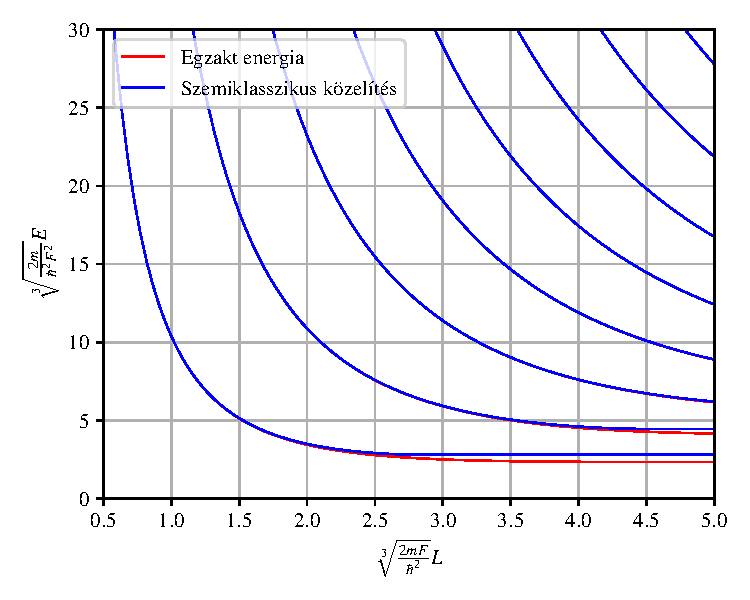
\includegraphics[scale=1]{./figs/energiaszintkozelites.pdf}
		\caption{Szemiklasszikus közelítés}
	\end{figure}
	
	\begin{figure}[H]
		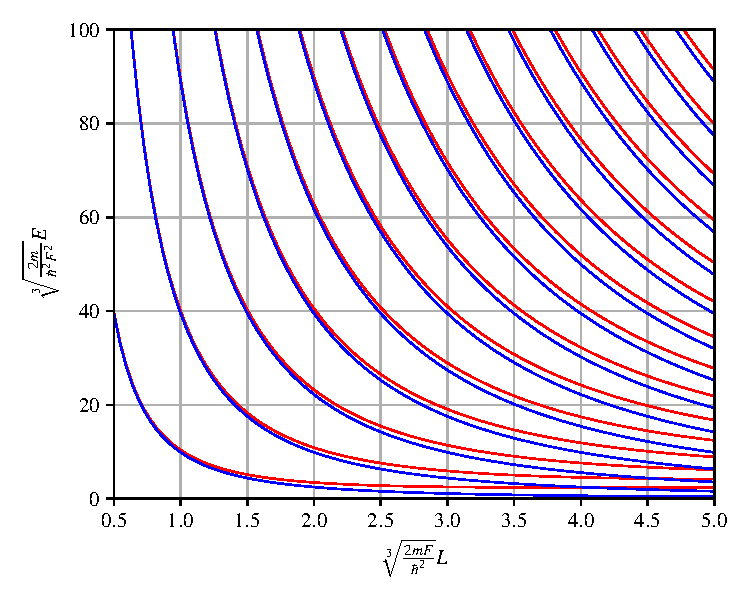
\includegraphics[scale=1]{./figs/infsquareenergia.pdf}
		\caption{Szemiklasszikus közelítés}
	\end{figure}

\section{Momentumok}
	
	
\section{Plafon érintés 1D}
	Azokat a parmaétereket keresem, ahol az alapállapot $E = FL$:
	\begin{equation}
		\Ti{\sqrt[3]{\frac{2mF}{\hbar^2}}L - \sqrt[3]{\frac{2m}{\hbar^2F^2}}FL} - \Ti{-\sqrt[3]{\frac{2m}{\hbar^2F^2}}FL} = 0
	\end{equation}
	, azaz
	\begin{equation}
		\Ai{-\sqrt[3]{\frac{2mF}{\hbar^2}}L} = 0
	\end{equation}
	. Az első gyöke az Airy függvénynek megadja azt az esetet, amikor az alapállapot ergiája $FL$, és nem pedig valamelyik gerjesztett állapoté.
	\begin{equation}
		-a_1 = \sqrt[3]{\frac{2mF}{\hbar^2}}L \approx 2.338
	\end{equation}



\section{3D doboz, ferde tér}
    A rendszer egy téglatest alakú dobozba zárt részecske. A doboz mérete $L_x$, $L_y$ és $L_z$. A dobozban homogén erőtér hat a részecskére, azaz $\boldsymbol{F} = const$. A potenciál így $V(x, y, z) = -\boldsymbol{F}_xx-\boldsymbol{F}_yy-\boldsymbol{F}_zz$. Mivel az a potenciál lineáris $x$ $y$ és $z$-ben, a Schrödinger egyenlet szeparálható.
    \begin{equation}
        \psi_{klm}\left(x, y, z\right) = \phi_k \left( x^\prime \right)\phi_l\left(y^\prime\right)\phi_m\left(z^\prime\right)
    \end{equation}
    Ahol $x^\prime = \sqrt[3]{\frac{2m\boldsymbol{F}_x}{\hbar^2}}x - \sqrt[3]{\frac{2m}{\hbar^2\boldsymbol{F}_x^2}}E_k$, $E_k$ pedig az 1 dimenziós probléma, $\Ti{\sqrt[3]{\frac{2m\boldsymbol{F}_x}{\hbar^2}}L - \sqrt[3]{\frac{2m}{\hbar^2\boldsymbol{F}_x^2}}E} - \Ti{-\sqrt[3]{\frac{2m}{\hbar^2\boldsymbol{F}_x^2}}E} = 0$, $k$. $\phi_k \left( x^\prime \right)$ az 1D-s rész TODO:REFERENCIA hullámfüggvénye. $y^\prime$, $z^\prime$, valamint $E_l$ és $E_m$ hasonlóan vannak definiálva a hozzájuk tartozó 1 dimenziós probléma alapján. A 3D-s hullámfüggvényhez tartozó energia az 1D-s megoldásokhoz tartozó energiák összege.
    \begin{equation}
        E = E_k + E_l + E_m
    \end{equation}
    Amennyiben valamelyik irányú komponense $\boldsymbol{F}$-nek 0, abban az esetben a hozzá tartozó 1D-s pprobléma a híres végtelen mély potenciálgödör, ahol
    \begin{equation}
        \phi_n = \sqrt{\frac{2}{L}}\sin\left(\frac{nx\pi}{L}\right)
    \end{equation}
    valamint
    \begin{equation}
        E_n = \frac{\hbar^2n^2}{2mL^2}
    \end{equation}
    
    TODO: ÁBRA AZ EGYSZER FÜGGŐLEGES ESET ENERGIÁIRÓL, esetleg szintén L függvényében.
    
    TODO: ábra 2D -quantum chaos in billiards-
    
    TODO: 2D (3D?) videó link időfelődésről
    
\section{Green függvény}
    
\section{Videó gyártás leírása}
    
    
    
\end{document}















